\documentclass[11pt]{article}
\usepackage[utf8]{inputenc}
\usepackage[french]{babel}
\usepackage[margin=3cm, paperwidth=21cm, paperheight=29.7cm]{geometry}
\usepackage{graphicx}
\usepackage{SIunits}
\usepackage{tabto}
\usepackage{eurosym}
\usepackage{subcaption}
\usepackage{hyperref}
\hypersetup{hidelinks}
\usepackage{url}
\usepackage{listings}
\usepackage[footnote]{acronym}
\usepackage[T1]{fontenc}
\usepackage{array}
\usepackage{titlesec}
\usepackage{todonotes}

\usepackage{fancyhdr}
\usepackage{caption}

\usepackage{xcolor}
 
\definecolor{codegreen}{rgb}{0,0.6,0}
\definecolor{codegray}{rgb}{0.5,0.5,0.5}
\definecolor{codepurple}{rgb}{0.58,0,0.82}
\definecolor{backcolour}{rgb}{0.95,0.95,0.92}
\definecolor{bluekeywords}{rgb}{0.13,0.13,1}
\definecolor{greencomments}{rgb}{0,0.5,0}
\definecolor{redstrings}{rgb}{0.9,0,0}
\definecolor{typedef}{rgb}{0.227, 0.49, 0.49}
\definecolor{violet}{rgb}{0.255, 0.2588, 0.5333}
\lstdefinestyle{C_Style}{
    language=C,
    backgroundcolor=\color{backcolour},   
    commentstyle=\color{codegreen},
    keywordstyle=\color{bluekeywords},
    numberstyle=\tiny\color{codegray},
    stringstyle=\color{codepurple},
    basicstyle=\ttfamily\footnotesize,
    breakatwhitespace=false,         
    breaklines=true,                 
    captionpos=b,                    
    keepspaces=true,                 
    numbers=left,                    
    numbersep=5pt,                  
    showspaces=false,                
    showstringspaces=false,
    showtabs=false,                  
    tabsize=2,
    emph={%  
    __mavlink_custom_struct_t, uint8_t, uint16_t, uint32_t, uint64_t, mavlink_custom_struct_t%
    },emphstyle={\color{typedef}}%
}

\lstdefinestyle{XML_Style}{
  language=XML,
  backgroundcolor=\color{backcolour},   
  commentstyle=\color{codegreen},
  keywordstyle=\color{bluekeywords},
  numberstyle=\tiny\color{codegray},
  stringstyle=\color{codepurple},
  basicstyle=\ttfamily\footnotesize,
  breakatwhitespace=false,         
  breaklines=true,                 
  captionpos=b,                    
  keepspaces=true,                 
  numbers=left,                    
  numbersep=5pt,                  
  showspaces=false,                
  showstringspaces=false,
  showtabs=false,                  
  tabsize=2,
  morekeywords={mavlink, message, enums, messages, wip, field, description, dialect, include},
  emph={  
    type, id, name, enum
    },emphstyle={\color{violet}}
}

\lstset{style=C_Style}
\pagestyle{fancy}
\lhead{STM32 Project} % controls the left corner of the header
\chead{} % controls the center of the header
\rhead{V2004} % controls the right corner of the header
\lfoot{} % controls the left corner of the footer
\cfoot{Page~\thepage} % controls the center of the footer
\rfoot{} % controls the right corner of the footer
\renewcommand{\headrulewidth}{0.4pt}
\renewcommand{\footrulewidth}{0.4pt}

\titleclass{\subsubsubsection}{straight}[\subsection]

\newcounter{subsubsubsection}[subsubsection]
\renewcommand\thesubsubsubsection{\thesubsubsection.\arabic{subsubsubsection}}
\renewcommand\theparagraph{\thesubsubsubsection.\arabic{paragraph}} % optional; useful if paragraphs are to be numbered


\titleformat{\subsubsubsection}
  {\normalfont\normalsize\bfseries}{\thesubsubsubsection}{1em}{}
\titlespacing*{\subsubsubsection}
{0pt}{3.25ex plus 1ex minus .2ex}{1.5ex plus .2ex}
\makeatletter

\titleclass{\subsubsubsubsection}{straight}[\subsection]

\newcounter{subsubsubsubsection}[subsubsubsection]
\renewcommand\thesubsubsubsubsection{\thesubsubsubsection.\arabic{subsubsubsubsection}}

\titleformat{\subsubsubsubsection}
  {\normalfont\normalsize\bfseries}{\thesubsubsubsubsection}{1em}{}
\titlespacing*{\subsubsubsubsection}
{0pt}{3.25ex plus 1ex minus .2ex}{1.5ex plus .2ex}
\makeatletter

\renewcommand\paragraph{\@startsection{paragraph}{6}{\z@}%
  {3.25ex \@plus1ex \@minus.2ex}%
  {-1em}%
  {\normalfont\normalsize\bfseries}}
\renewcommand\subparagraph{\@startsection{subparagraph}{7}{\parindent}%
  {3.25ex \@plus1ex \@minus .2ex}%
  {-1em}%
  {\normalfont\normalsize\bfseries}}
\def\toclevel@subsubsubsection{4}
\def\toclevel@subsubsubsubsection{5}
\def\toclevel@paragraph{6}
\def\toclevel@paragraph{7}
\def\l@subsubsubsection{\@dottedtocline{4}{7em}{4em}}
\def\l@subsubsubsubsection{\@dottedtocline{5}{10em}{5em}}
\def\l@paragraph{\@dottedtocline{6}{13em}{6em}}
\def\l@subparagraph{\@dottedtocline{7}{17em}{7em}}
\makeatother

\setcounter{secnumdepth}{5} % Profondeur des nombres des titres
\setcounter{tocdepth}{3}

\renewcommand{\contentsname}{Summary}
\begin{document}
\thispagestyle{plain}% Removes the header from the first page. Change plain to empty to remove the numbering entirely.

\begin{titlepage}

  \newcommand{\HRule}{\rule{\linewidth}{0.5mm}} % Defines a new command for the horizontal lines, change thickness here
  
  \center % Center everything on the page
   
  %----------------------------------------------------------------------------------------
  %	HEADING SECTIONS
  %----------------------------------------------------------------------------------------
  
  %\textsc{\LARGE University Name}\\[1.5cm] % Name of your university/college
  %\textsc{\Large Major Heading}\\[0.5cm] % Major heading such as course name
  %\textsc{\large Minor Heading}\\[0.5cm] % Minor heading such as course title
  
  %----------------------------------------------------------------------------------------
  %	TITLE SECTION
  %----------------------------------------------------------------------------------------
  
  \HRule \\[0.4cm]
  { \huge \bfseries Rapport \textsc Alternance Master SME  }\\[0.4cm] % Title of your document
  { \LARGE Première année}\\[0.4cm] % Title of your document
  \HRule \\[1.5cm]
   

  %----------------------------------------------------------------------------------------
  %	AUTHOR SECTION
  %----------------------------------------------------------------------------------------
  
  %\begin{minipage}{0.4\textwidth}
  %\begin{flushleft} \large
  %\emph{Author:}\\
  %John \textsc{Smith} % Your name
  %\end{flushleft}
  %\end{minipage}
  %~
  %\begin{minipage}{0.4\textwidth}
  %\begin{flushright} \large
  %\emph{Supervisor:} \\
  %Dr. James \textsc{Smith} % Supervisor's Name
  %\end{flushright}
  %\end{minipage}\\[2cm]
  
  % If you don't want a supervisor, uncomment the two lines below and remove the section above
  \Large
  Etudiant : Cyprien \textsc{Quivet}\\ % Your name
  \Large
  Tuteur : Nicolas  \textsc{Roddier}\\ % Your name
  
  %----------------------------------------------------------------------------------------
  %	DATE SECTION
  %----------------------------------------------------------------------------------------
  
  
  %----------------------------------------------------------------------------------------
 % \vfill % Fill the rest of the page with whitespace
  %	LOGO SECTION
  %----------------------------------------------------------------------------------------


  \begin{figure}[b]
    \centering
    
\includegraphics{img/LogoTachyssema.png}\\[1cm] % Include a department/university logo - this will require the graphicx package
    \label{fig:LogoTachyssema}
  \end{figure}
  {\Large Avril 2020}\\[2cm] % Date, change the \today to a set date if you want to be precise

  
   
  %----------------------------------------------------------------------------------------
  
  \end{titlepage}
\newpage
\setcounter{page}{2}

\renewcommand{\thepage}{\arabic{page}}

\tableofcontents
\newpage

\newpage

\section{Présentation de mon projet de M2 }

Dans cette partie nous nous interesserons à mon projet de deuxième année d'alternance que je commence à mener dès cette année en parallèle de mes autres projets en cours. 

\subsection{Présentation}

Mon projet de M2 consiste à la réalisation d'un boitier compatible avec les rails DIN, intégrant un FPGA permettant de réaliser diverses opérations de traitements. L'objetif fixé est de concevoir la carte PCB qui acceuillera les élements électroniques ainsi que la partie mécanique qui correspond au boitier tout en répondant à toutes les normes en vue d'une commercialisation sur le marché. 

\subsection {Pourquoi réaoiser ce projet ? } 

L'interêt de la mise en oeuvre d'un tel boitier est de pouvoir répondre à un besoin client important. En effet ce boitier pouvant s'adapter sur un rail DIN pourra être utilisé pour réaliser des opérations (traitement vidéo, calculs spécifiques ..) que les autres équipements ne peuvent pas réaliser.

Par exemple si on prend le cas d'un automate qui possède une puissance de calculs limitée. Les données à traiter sont transmises au boitier contenant le FPGA, traitées puis renvoyées dans l'automate. 

\subsection {Cahier des charges } 

Le projet doit répondre à un cahier des charges précis : 
\newline
\begin{itemize}
	\item Le boitier doit être compatible avec les rails DIN.
	\item La carte pcb doit être optimisée pour le boitier. Les contours de la carte seront établis en fonction de la forme du boitier.
	\item La carte électronique pourra être programmée par le biais d'un port USB.
	\item La carte électronique disposera de 4 connecteurs SFP qui pourront servir d'entrées ou de sortie.
	\item Le projet devra répondre au normes de comptatibilités électroniques.
	\item Le projet devra répondre au normes CE en vue d'une commercialisation. 

\end{itemize}


\subsection {Réalisation du boitier } 

Dans un premier temps j'ai commencé la réalisation du boitier qui acceuillera la carte pcb. Phoenix Contact est un fabriquant de solutions industrielles qui propose également un service de personnalisation de boitier industriels. Ce service laisse un libre choix aux clients en ce qui concerne les types de boitiers souhaités, les dimensions du boitier ainsi que le choix des connecteurs utilisés.
\newline
Dans un premier temps, j'ai donc réalisé sur le site de Phoenix Contact un boitier compatible rail DIN répondant au exigences du cahier des charges. Une fois la configuration terminée, Phoenix Contact fournit le modèle 3D du boitier : 
\newpage
\begin{figure}[ht]
    \centering
    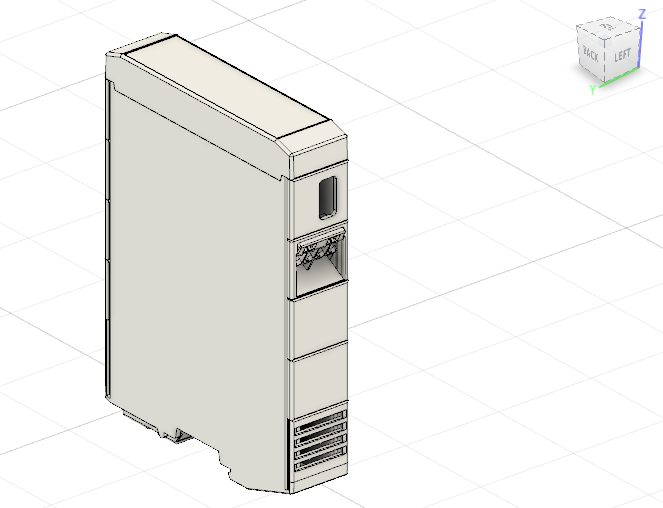
\includegraphics[scale=0.35]{img/boitier.PNG}
    \caption{Apperçu de la conception 3D du boitier }
    \label{fig:CameraCmdsettings}
\end{figure}

On peut également voir que les contours de la carte PCB sont eux aussi générés par le site web : 

\begin{figure}[ht]
    \centering
    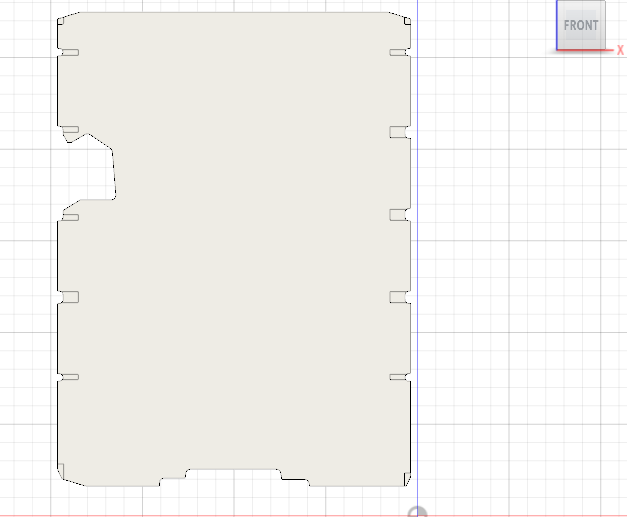
\includegraphics[scale=0.45]{img/pcb.PNG}
    \caption{Apperçu de la conception 3D du boitier }
    \label{fig:CameraCmdsettings}
\end{figure}




\clearpage

\end{document}